%% Author_tex.tex
%% V1.0
%% 2012/13/12
%% developed by Techset
%%
%% This file describes the coding for rsproca.cls

\documentclass[]{rsos}%%%%where rsos is the template name


\usepackage[T1]{fontenc}
\usepackage[utf8]{inputenc}


% tightlist command for lists without linebreak
\providecommand{\tightlist}{%
  \setlength{\itemsep}{0pt}\setlength{\parskip}{0pt}}

% From pandoc table feature
\usepackage{longtable,booktabs,array}
\usepackage{calc} % for calculating minipage widths
% Correct order of tables after \paragraph or \subparagraph
\usepackage{etoolbox}
\makeatletter
\patchcmd\longtable{\par}{\if@noskipsec\mbox{}\fi\par}{}{}
\makeatother
% Allow footnotes in longtable head/foot
\IfFileExists{footnotehyper.sty}{\usepackage{footnotehyper}}{\usepackage{footnote}}
\makesavenoteenv{longtable}



%%%% *** Do not adjust lengths that control margins, column widths, etc. ***

%%%%%%%%%%% Defining Enunciations  %%%%%%%%%%%
\newtheorem{theorem}{\bf Theorem}[section]
\newtheorem{condition}{\bf Condition}[section]
\newtheorem{corollary}{\bf Corollary}[section]
%%%%%%%%%%%%%%%%%%%%%%%%%%%%%%%%%%%%%%%%%%%%%%%

\begin{document}


%%%% Article title to be placed here
\title{Supplementary Inforamtion}

\author{
Carmen Cabrera$^{1}$,
Francisco Rowe$^{1}$}

\address{
  $^{1}$Geographic Data Science Lab, Department of Geography and Planning, University of Liverpool, Liverpool, United Kingdom.\\
  $^{}$}
%%%% Subject entries to be placed here %%%%
\subject{
subject 1,
subject 2,
subject 3}

%%%% Keyword entries to be placed here %%%%
\keywords{
one,
two,
optional,
optional,
optional}

%%%% Insert corresponding author and its email address}
\corres{
  Carmen Cabrera\\
  e-mail: \href{mailto:C.Cabrera@liverpool.ac.uk}{\nolinkurl{C.Cabrera@liverpool.ac.uk}}
}

%%%% Abstract text to be placed here %%%%%%%%%%%%
\begin{abstract}
The abstract text goes here. The abstract text goes here. The abstract text goes here. The abstract text goes here. The abstract text goes here. The abstract text goes here. The abstract text goes here. The abstract text goes here.
\end{abstract}
%%%%%%%%%%%%%%%%%%%%%%%%%%%

\providecommand{\EndFirstPage}{%
}

\maketitle

The main document should include:

Title (no more than 150 characters)

Author names and affiliations, and ORCID iDs where available

Abstract (no more than 200 words). (This will be used in reviewer
invitation emails so please think about how to describe your work to
make it easy for a potential reviewer to determine whether they would be
suitable.)

All main manuscript text. Ensure that all figures, tables and any
relevant supplementary materials are mentioned within the text
References

Acknowledgements and funding statement (ensure that you have included
grant numbers and the names of any funding providers)

Tables with captions Figure captions with credits where relevant

\newpage

\hypertarget{introduction-fr}{%
\section{Introduction (FR)}\label{introduction-fr}}

Technological advances in computational power, storage and digital
network platforms have unleashed a data revolution producing large
trails of digital trace data containing location information. These data
have revolutionised research and business activities offering novel
opportunities to understand human behaviour and processes
\citep{rowe23-bigdata}. Digital trace data offer high spatial granularity,
geographic coverage, high temporal frequency and instant information to
capture and understand human activities at unprecedentedly high
resolution and scale, and produce actionable intelligence in real time
to support rapid decision making. Digital trace data have been used for
a range of applications, such monitoring footfall changes {[}REF{]},
inferring mobility signatures {[}REF{]}, sensing land use patterns {[}REF{]},
predicting socioeconomic levels {[}REF{]}, defining urban extents {[}REF{]} and
estimating population displacement {[}REF{]}.

However, the use of digital trace data present major epistemological,
methodological and ethical challenges \citep{rowe23-bigdata}. A key
unresolved challenge is the potential presence of biases in digital
trace data to compromise their statistical representativeness and
perpetuate social injustice {[}REF{]}. Biases reflect societal digital and
socioeconomic inequalities. Biases emerge from differences in the access
and use of the particular digital technology used to collect data, such
as mobile phone applications \citep{wesolowski13-biases}. Only a fraction of
the population in an area owns a mobile phone, and even an smaller share
actively use a specific mobile phone app. In the UK, for example, 98\% of
the adult population have a mobile phone and 92\% of this population use
a smartphone \citep{ofcom23}, but a smaller percentage actively use Facebook
(70\%) or Twitter (23\%) \citep{statista24}. Additionally, biases emerge from
differences in the access and use of digital technology across
population subgroups according to their socioeconomic and demographic
profile. For instance, wealthy and urban populations tend to be
over-represented in mobile phone data {[}REF{]} and of digital social
platforms, such as Facebook {[}REF{]} and Twitter/X {[}REF{]}.

The use of biased digital trace data can thus have major practical and
societal implications.

As a result, population statistics derived from digital trace data
cannot provide population-level representation. They can only offer
rough signals about the spatial distribution of (e.g.~spatial
concentration), trends (e.g.~increasing) and changes (e.g.~low to high)
in populations \citep{rowe22-sensing-ukraine}.

and amplify socioeconomic disparities

Gaps:

Aim: We propose an approach to measure biases -

Research questions:

Contribution:

Structure:

Efforts have been made to correct these biases through two general
approaches. A first general approach consists in adjusting DF-derived
population counts from social media by developing correction factors
(e.g. \citep{yildiz17-twitter}, \citep{Hsiao24-bias}). Correction factors are
often estimated as the ratio of active social media users to census
population counts by demographic attributes (e.g.~age). The principles
are similar to survey post-stratification methods i.e.~to make
DF-derived population counts representative of the census populations.
However, a key data requirement of this approach is on having data on
population by attribute, but such data are generally unavailable from
DFs. Only information on location, time and total active users is
recorded. As such, this approach cannot be generalised to different DFD
sources and geographical contexts, and when applied on total population
counts, biases associated with demographic and socioeconomic user
attributes are not corrected (e.g. \citep{rodriguez-carrion18-biases},
\citep{schlosser21-biases}, \citep{pak22-correcting-bias}). A second approach uses
a regression modelling approach. Intuitively this approach produces
representative population counts by explicitly measuring and removing
the sources of biases in the data \citep{kramer-schadt13-bias-correction}.
This approach has primarily been used in Ecology to obtain
representative population distributions of animal species
\citep{zizka21-sampbias}, but it has not been used in the context of DFD. In
recent work, the PI adopted a similar approach to correct multiple
sources of biases in census data to produce bias-adjusted migration
estimates \citep{aparicio-castro23-bayesian}. DEBIAS builds on this work to
develop a general framework and software package aiming to correct
biases in origin-destination mobility counts derived from DFs in the
absence of demographic and socioeconomic information on users of digital
platforms.

\hypertarget{data-and-methods}{%
\section{Data and methods}\label{data-and-methods}}

\hypertarget{data-cca}{%
\subsection{Data (CCA)}\label{data-cca}}

\hypertarget{facebook}{%
\subsubsection{Facebook}\label{facebook}}

We use anonymised aggregate location data from Facebook app users who
have the location services setting turned on on their smartphone for the
UK, covering March 2021, the month when the 2021 UK Census was carried
out. We use the Facebook Population dataset created by Meta and accessed
through their Data for Good Initiative
(\url{https://dataforgood.facebook.com}). Prior to releasing the datasets,
Meta ensures privacy and anonymity by removing personal information and
applying privacy-preserving techniques {[}@Maas19{]}. Small-count dropping
is one of these techniques. A data entry is removed if the population or
movement count for an area is lower than 10. The removal of small counts
may mean that population counts in small sparsely populated areas are
not captured. A second technique consists in adding a small undisclosed
amount of random noise to ensure that it is not possible to ascertain
precise, true counts for sparsely populated locations. Third, spatial
smoothing using inverse distance-weighted averaging is also applied is
applied to produce a smooth population count surface.

The Facebook Population dataset offers information on the number of
active Facebook users in a spatial unit at a given point in time. The
data is temporally aggregated into three daily 8-hour time windows (i.e.
00:00-08:00, 08:00-16:00 and 16:00- 00:00). In this work, we are
interested in capturing resident population, so we consider only data
corresponding to the time window corresponding to the night-time hours
(00:00-08:00).

The Facebook Population dataset is spatially aggregated according to the
Bing Maps Tile System developed by Microsoft (Microsoft). The Tile
System is a geospatial indexing system that partitions the world into
tile cells in a hierarchical way, comprising 23 different levels of
detail (Microsoft). At the lowest level of detail (Level 1), the world
is divided into four tiles with a coarse spatial resolution. At each
successive level, the resolution increases by a factor of two. The data
that we used are spatially aggregated into Bing tile levels 13. That is
about 4.9 x 4.9km at the Equator {[}@Maas19{]}. In the next steps, we
compare the Facebook Population data with UK census data. To facilitate
this comparison, we aggregate the data into administrative units,
specifically UK Local Authority Districts (LADs).

\hypertarget{twitter}{%
\subsubsection{Twitter}\label{twitter}}

We use an anonymised, openly available, analysis-ready dataset of active
Twitter users in the UK. The data is derived from X (previously Twitter)
in the form of monthly active user counts residing across the UK
geography. The dataset is based on tweets from UK users \citep{wang2022}
collected via the Twitter Academic API. These tweets are either
geolocated at the time of posting or manually geocoded using a bounding
box provided by the Twitter Academic API, based on the IP address of the
posting device. The full dataset includes 161 million tweets from
February 2019 to December 2021; however, we focus on data from March
2021 to align with the 2021 UK Census. Users' Local Authority District
(LAD) of residence is identified using a frequency-based home-location
algorithm. Further details on the dataset's methodology can be found in
\citep{wang2022} .

While the X Academic API is no longer available to download data, but
existing and future projects offer an opportunity for research based on
X data. Global repositories of historical geolocated tweet data are
accessed through the Internet Archive (1996) and Harvard Geotweet
Archive (\url{https://gis.harvard.edu/data}). Despite these limitations, we
consider X data as it remains a key source of historical digital trace
data.

\hypertarget{multi-app-gps-data}{%
\subsubsection{Multi-app GPS data}\label{multi-app-gps-data}}

The data used in this study were sourced by a data analytics company
that collects GPS location data from around 26\% of smartphones in the
UK. The raw data is collected for individual anonymised devices, from
numerous smartphone applications where the users have explicitly granted
location-sharing permissions. The full dataset covers 7 days
corresponding to the first week of April for the UK, including X GPS
records and X unique devices. While the dates covered by dataset do not
exactly coincide with the 2021 UK Census dates, the alignment is very
close.

We process the data to estimate users' place of residence by assuming
that the residence of a device owner corresponds to the location with
the highest number of GPS records during night hours (11 PM -- 7 AM). For
a location to be classified as a residence, it must account for more
than 50\% of recorded nighttime locations and be visited at least twice.
To ensure consistency in our analysis when comparing with other data
sources, we aggregate these residence locations at the Local Authority
District (LAD) level.

\hypertarget{methods}{%
\subsection{Methods}\label{methods}}

In this section, we outline our proposed methodology, which consists of
two interconnected stages aimed at quantifying two types of biases:
coverage biases and representational biases. Coverage biases relate to
the sample size of the dataset and refer to the proportion of the
population covered in the dataset. Representational biases, arise from
the demographic and socioeconomic characteristics of the users who
generate the digital trace data through specific technologies.

In the first stage of our methodology, we focus on quantifying coverage
biases by examining the variations in coverage across different spatial
units. We leverage the spatial granularity of digital trace data to
analyse coverage biases at more localised spatial scales. This allows us
to identify the extent to which different regions are represented within
the datasets, revealing any potential underrepresentation or
overrepresentation in specific locations.

In the second stage, we focus on quantifying representational biases. To
do this, we leverage the spatial heterogeneity of coverage biases and
model this variation in terms of demographic and socioeconomic variables
that characterise local populations. This analysis allows us to identify
which specific demogrpahic and socioeconomic population attributes, such
as average income, education level or age composition, are more likely
to be associated with higher values of coverage bias, thus highlighting
which population groups tend to be underrepresented in different sources
of digital trace data.

\hypertarget{measuring-coverage-bias-cca}{%
\subsubsection{Measuring coverage bias (CCA)}\label{measuring-coverage-bias-cca}}

We define a metric to quantify the magnitude of coverage bias in each
subnational area. This metric is based on the population coverage of the
dataset, which we compute as the ratio of the population captured
(sample size) by dataset \(D\), denoted as \(P_i^D\), to the total local
population of an area, \(P_i\). Formally, the coverage \(c_i\) is given by:
\begin{equation}
c_i = \dfrac{P_i^D}{P_i} \times 100,
\end{equation} where \(D\) identifies a given dataset, and \(i\) denotes
each subnational area. The resulting ratio \(c_i\) is assumed to take
values between \(0\) and \(100\), with 100 representing full population
coverage. If users have multiple accounts, the ratio can exceed \(100\),
since the total sample size could be greater than the local population
of area \(i\).

We then define the size of bias \(e_i\) as:

\begin{equation} \label{eq:size-bias}
e_i = 100 - c_i
\end{equation}

In this case, a value of \(e_i = 0\) indicates a lack of coverage bias,
which corresponds to full population coverage (\(c_i = 100\)). We use this
bias indicator to analysis the magnitude and spatial distribution of
coverage bias across multiple sources of digital trace data.

\hypertarget{assessing-the-driving-factors-of-bias-fr}{%
\subsubsection{Assessing the driving factors of bias (FR)}\label{assessing-the-driving-factors-of-bias-fr}}

We seek to understand the association between the size of bias and
area-level demographic and socioeconomic attributes. To what extent
different demographic and socioeconomic groups are represented in DFD?
And how do these vary geographically and across digital platform? We
will assess these questions by measuring the area-level association
between our coverage indicator and key demographic and socioeconomic
attributes. We will use a random forest to model our coverage indicator
as a function of demographic and socioeconomic attributes. The outcomes
will identify the most important area-level demographic and
socioeconomic features to predict the coverage bias of a given digital
technology. We will use this information to inform our models in WP-II.

eXtreme Gradient Boosting (XGBoost) is an efficient and scalable
implementation of gradient boosting framework by \citep{friedman2001, friedman2000}.

\hypertarget{results}{%
\section{Results}\label{results}}

\hypertarget{varying-extent-of-bias-across-data-sources}{%
\subsection{Varying extent of bias across data sources}\label{varying-extent-of-bias-across-data-sources}}

As digital trace data becomes increasingly accessible, it opens up new
avenues for studying human behaviours with remarkable temporal and
spatial precision, extensive geographic coverage, and near real-time
access. However, the potential presence of biases can undermine the
validity of the data to deliver statistically representative evidence.

In this section, we focus on quantifying the biases in multiple sources
of digital trace data that arise due to the extent of population
coverage, i.e.~the proportion of the total population captured in the
dataset. In Figure , we contextualise these findings by comparing them
with various traditional datasets, particularly key UK surveys available
through the UK Data Service \citep{ukdataserviceSurveysData}. On the
\(x\)-axis, we represent two variables: at the top, the sample size of the
dataset, expressed as the number of respondents or subjects per 1,000
people, which reflects the population coverage of the dataset; and at
the bottom, a measure of bias in terms of this coverage, as defined in
equation \ref{eq:size-bias}. The figure highlights the remarkable
ability of digital trace data to capture a larger share of the total
population compared to traditional surveys, thanks to the automated,
passive nature of data collection on digital platforms. This contrasts
with the manual recruitment and data collection processes required for
surveys. As a result, the size of bias is generally lower for digital
trace data, highlighting its potential to inform comprehensive empirical
analyses.

\begin{figure}
\hypertarget{fig:survey}{%
\centering
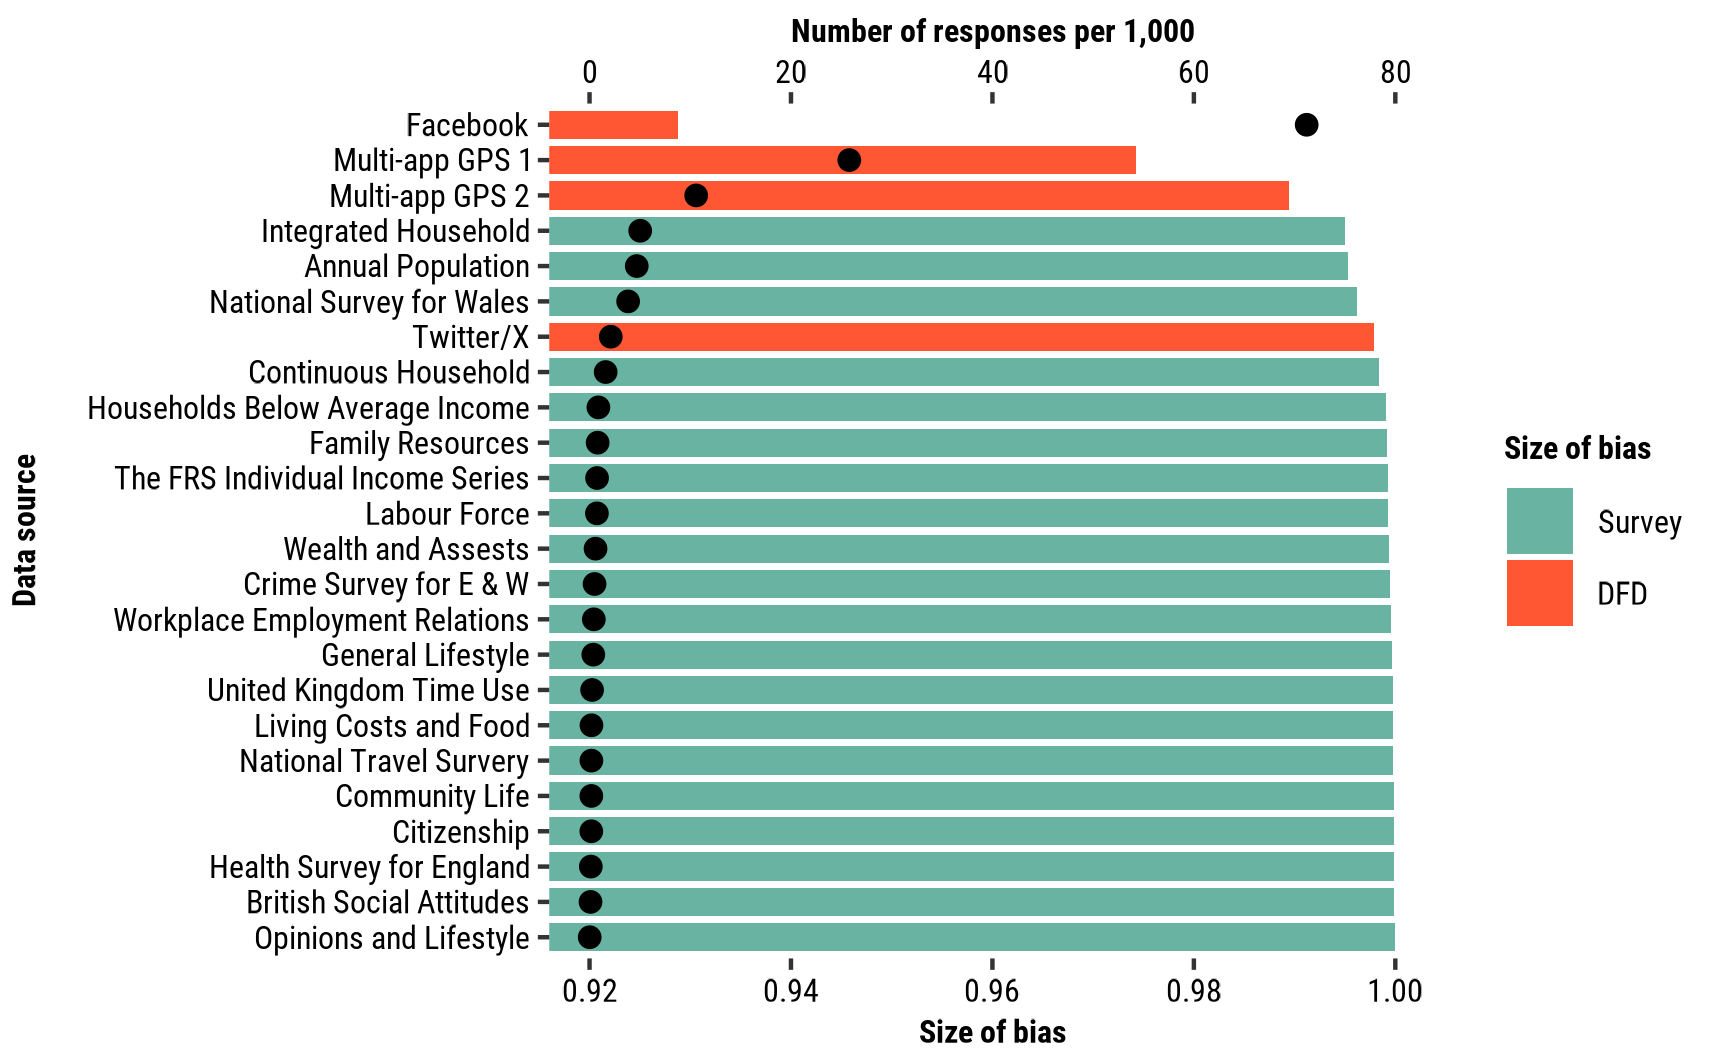
\includegraphics{figures/compare-surveys-two-axis.png}
\caption{Size of bias and population coverage (per 1,000 population) by data
source.}\label{fig:survey}
}
\end{figure}

While the findings in Figure \ref{fig:survey} demonstrate the potential
of digital trace data compared to traditional data sources, high
population coverage alone does not ensure the data is representative of
different population groups.

In surveys, specific strategies are usually implemented during the data
generation process to improve the statistical representativeness of the
sample. For example, sampling techniques such as stratified sampling or
cluster sampling can be applied so that the sample reflects the broader
population of interest. After sampling, if certain groups remain
under-represented, responses can be adjusted using post-stratification
techniques. However, even when these strategies are applied, there is no
guarantee that the survey will be fully representative of the broader
population of interest \citep{cochran1977sampling}. This is because
representativeness can only be achieved with respect to a finite set of
attributes (e.g.~age, gender, income levels, location, etc.). Ensuring
perfect representativeness would only be possible either by surveying
the whole population.

With digital trace data, achieving statistical representativeness is
even more challenging. Unlike survey data, which is actively collected
using structured sampling methods, digital trace data is generated
passively as a byproduct of online interactions, transactions, or device
usage, without any control over who is included in the dataset.
Furthermore, by the time this data reaches researchers or analysts, it
is often anonymised, and does not contain demographic identifiers. As a
result, it is not possible to apply the standard post-stratification
weighting techniques that are typically used to adjust survey or census
data for improved representativeness.

We argue that, even though we do not always have specific demographic
information of the individuals captured through digital trace data, we
can infer some of these characteristics by leveraging the
spatio-temporal granularity of digital trace data. We argue that this is
a necessary first step to understand which population groups might be
under or over-represented in different sources of digital trace data.
This information is necessary to later adjust the data so that it is
more representative of the population of interest.

\hypertarget{the-spatial-distribution-of-biases-cca}{%
\subsection{The spatial distribution of biases (CCA)}\label{the-spatial-distribution-of-biases-cca}}

Next, we take advantage of the detailed geographic information in the
digital trace data to analyse bias at smaller, more localised spatial
levels. This helps us understand how well different geographic areas are
represented in the datasets. Since local populations vary in their
socioeconomic characteristics, we can use the degree of bias at these
smaller scales in the next step of our analysis, to determine which
population attributes are most associated with underrepresentation in
the data.

Figure \ref{fig:size-bias-spatial} shows the geographic variation of the
size of bias at the Local Authority District (LAD) level. Each row in
the figure corresponds to each of the digital trace datasets analysed
here. Within each row, we include: i) an hexagonal cartogram for the
size of bias in each LAD, representing the LADs as hexagons of equal
size to simplify the visualisation while maintaining relative positions;
with this cartogram, we report Moran's I as a measure of spatial
autocorrelation and its associated p-value, ii) a histogram of the size
of bias, showing the distribution of values across LADs, iii) a scatter
plot of the population covered by the digital trace data vs.~the actual
population of each LAD; with the scatter plot, we include the Pearson
correlation coefficient and its associated p-value.

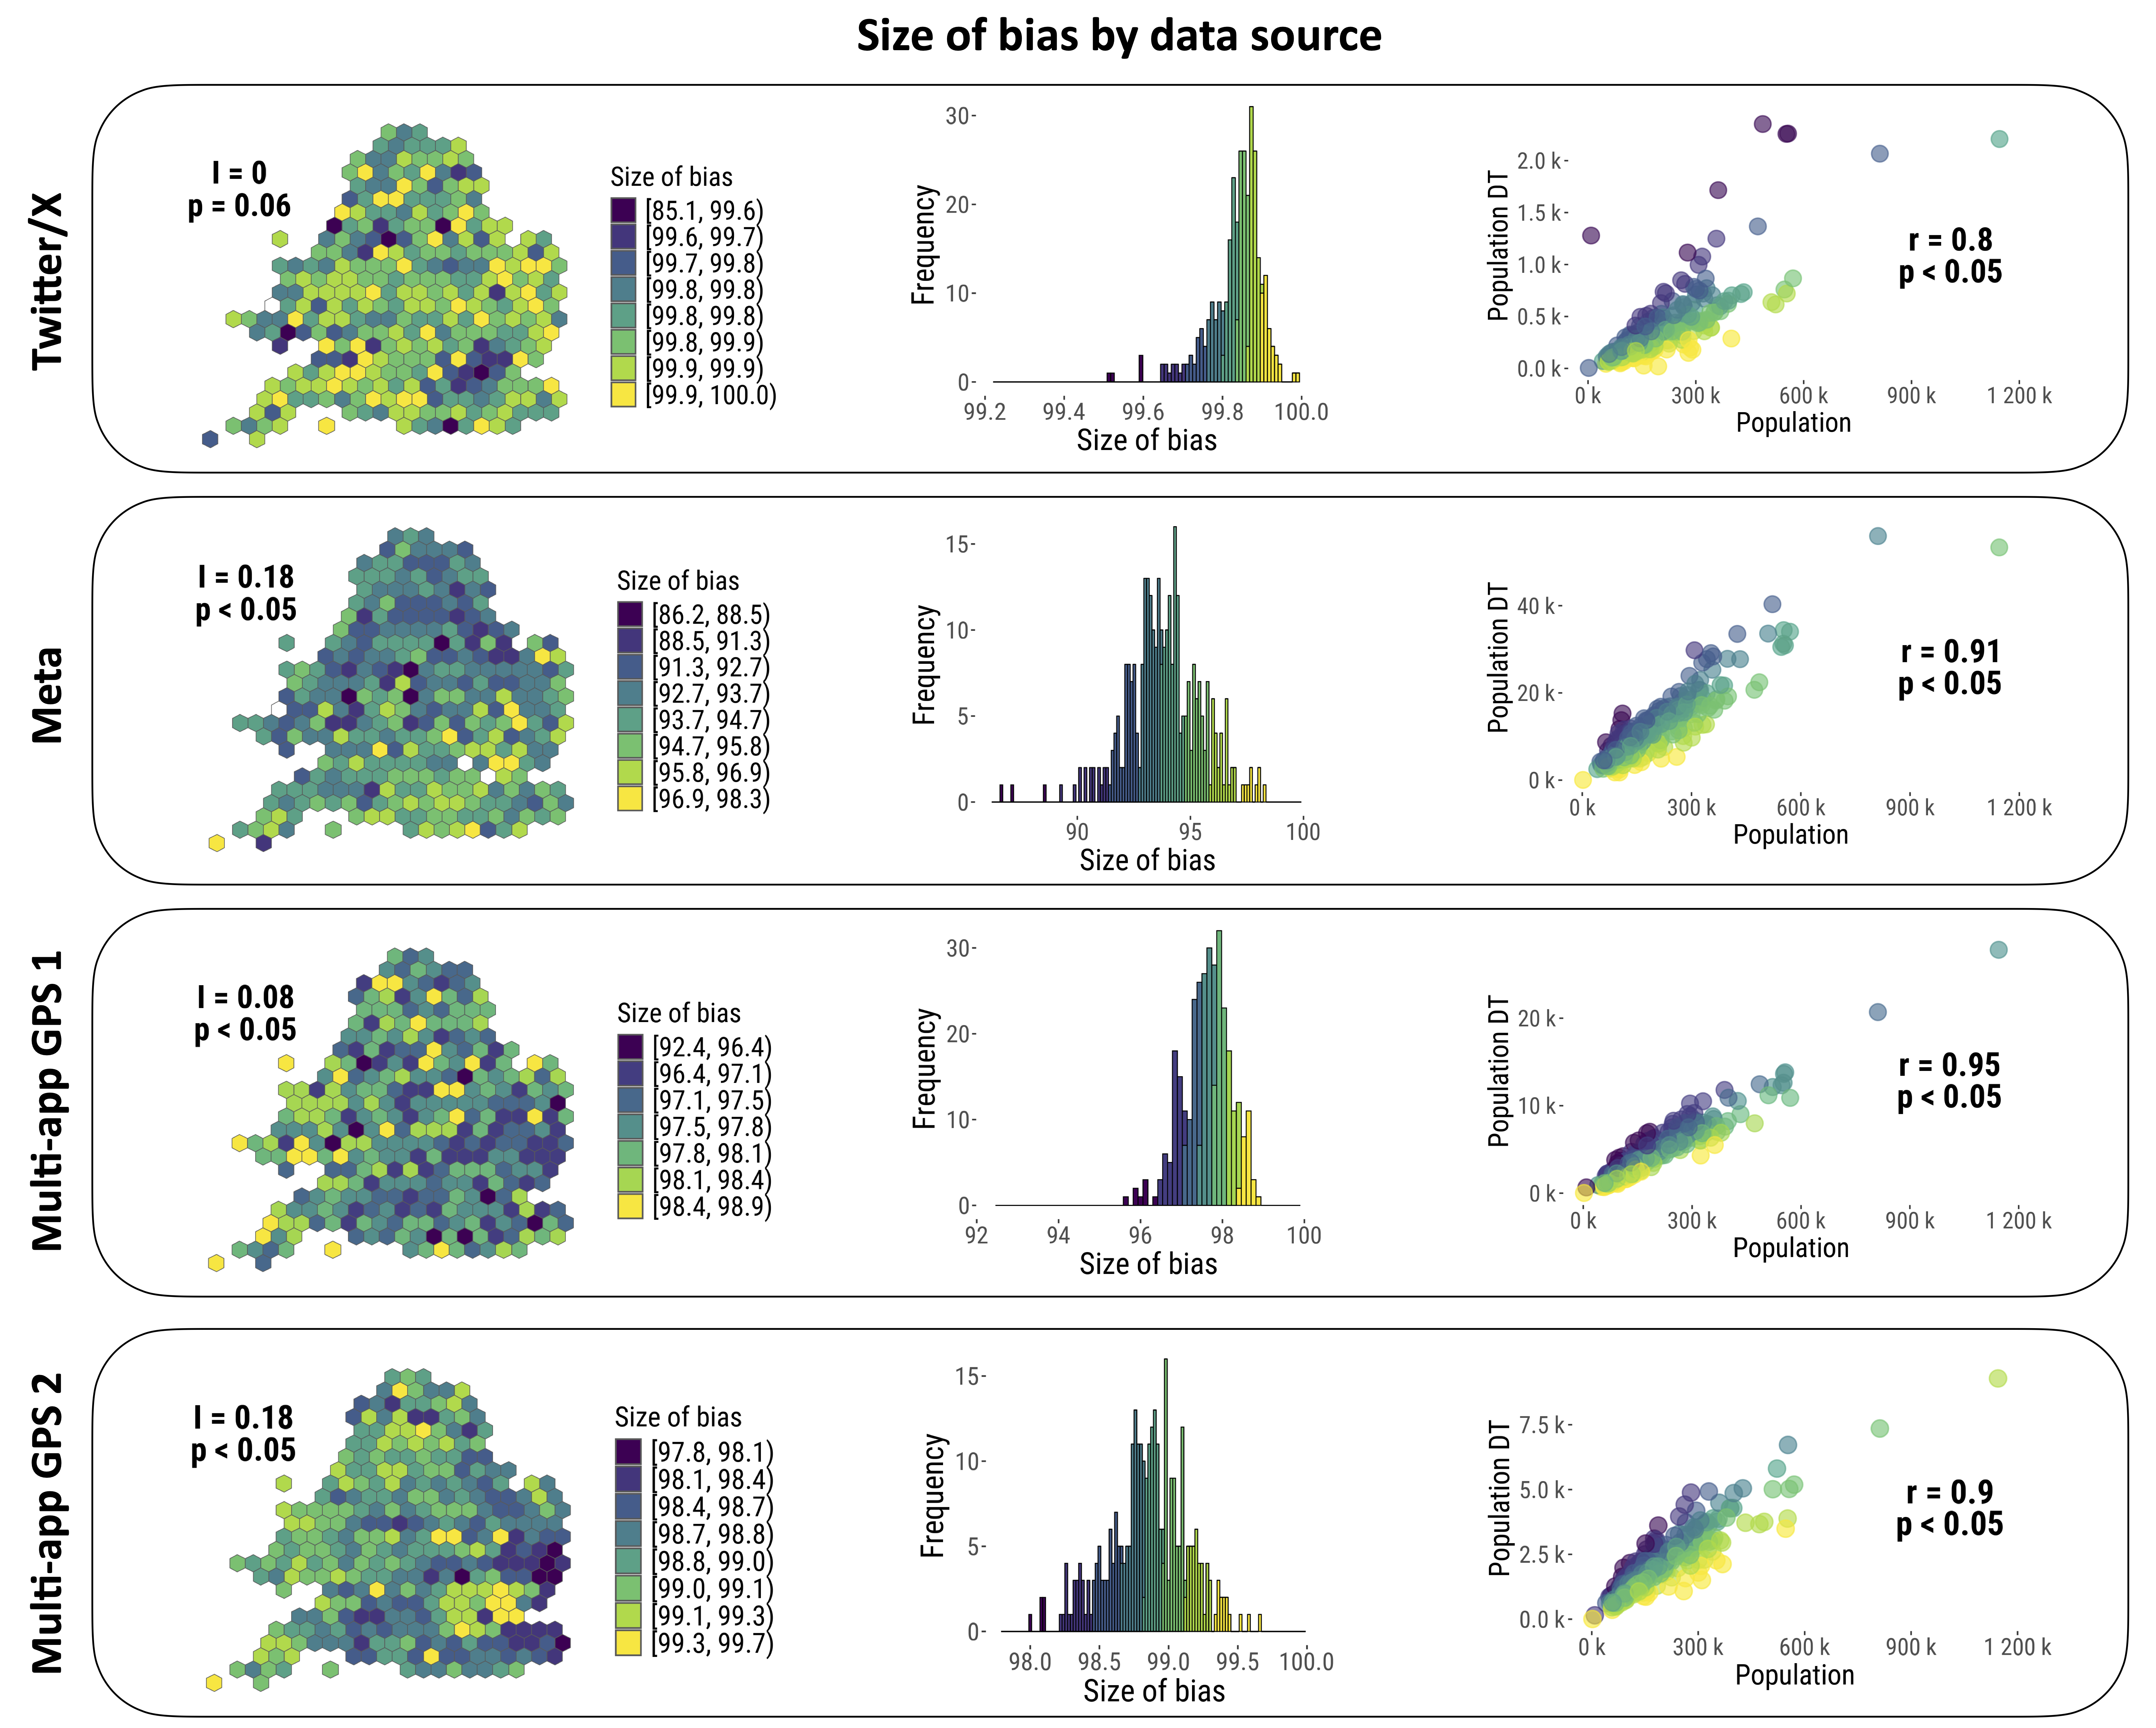
\includegraphics[width=5.55208in,height=4.35417in]{figures/Fig-size-bias.png}

Examining the spatial variation in bias size, we observe distinct
patterns across the DT datasets considered. These varied spatial
patterns likely stem from differences in the demographic composition of
users for each technology. Factors such as age, socioeconomic status,
digital literacy, and regional preferences for certain platforms or
devices may contribute to these variations. Bias tends to display
stronger spatial patterns for Meta data and the second source of
multi-app GPS data, with lower bias in the North of England and Wales.
In contrast, Twitter/X data and the first souce of multi-app GPS data
follow more mixed patterns, as demonstrated by the values of Moran's I
closer to zero. Twitter/X data generally exhibits high bias, except in
London, the South East, and a few isolated areas. Similarly, bias in
first source of multi-app data tends to be lower in the South and South
East.

Turning to the histograms, we observe that bias size is highest for
Twitter/X data, with all values exceeding 99.5 except for a single
outlier, the City of London. This outlier likely arises due to the
unique demographic and occupational characteristics of the area. While
relatively few people reside in the City of London, it hosts a large
number of workers, including temporary professionals, who may be staying
in hotels. The home-detection algorithm in \citep{wang2022} used to generate
the Twitter/X data used here might classify the workplace or temporary
accommodations of City of London workers as their primary residences,
leading to an anomalously low bias measurement. Following Twitter/X, the
second source of multi-app GPS data exhibits the next highest bias
values. In contrast, the first source of multi-app data shows lower
bias, while Meta data has the lowest overall bias. Notably, Meta data
also displays the widest distribution of bias values, indicating greater
variability across different locations.

The scatter plots show a high linear correlation between the population
covered by the digital trace data and the actual population of each LAD,
as demonstrated by the Pearson coefficient, all above 0.8. This suggests
that, on average, the actual population in the LADs is not an indicator
of the size of bias in DT data, as the population coverage \(c_i\) remains
the consistent regardless of \(P_i\) . This could be a result of the fact
that the biases in the data are not driven by the number of people, but
rather by other their demographic characteristics such as age, income or
educational level. In the next section, we explore the variability of
demographic attributes of local populations as possible determinants of
the size of bias.

\hypertarget{explaining-biases-fr}{%
\subsection{Explaining biases (FR)}\label{explaining-biases-fr}}

\hypertarget{discussion-fr}{%
\section{Discussion (FR)}\label{discussion-fr}}

\hypertarget{conclusion-cca}{%
\section{Conclusion (CCA)}\label{conclusion-cca}}

\ethics{Please provide details on the ethics.}

\dataccess{Please provide details on the data availability.}

\aucontribute{Please provide details of author contributions here.}

\competing{Please declare any conflict of interest here.}

\funding{Please provide details on funding}

\disclaimer{Please provide disclaimer text here.}

\ack{Please include your acknowledgments here, set in a single paragraph. Please do not include any acknowledgments in the Supporting Information, or anywhere else in the manuscript.}

\bibliographystyle{RS}
\bibliography{sample.bib}


\end{document}
